\chapter{Dark Matter}
\begin{center}
{\small \it (send feedback on this chapter to \href{mailto:s4_de@cosmo.uchicago.edu}{s4\_de@cosmo.uchicago.edu})}
\end{center}
%  currently spit off into its own chapter we may remerge them when sections are more complete
%We have learned from many different experiments (weak and strong lensing, studies of the Bullet Cluster, the Cosmic Microwave Background, etc) that approximately $84\%$ of all the matter in the universe is composed of dark matter, which is not accounted for by the Standard Model of particles. However, the particle nature of dark matter remains unknown, and light particles like axions, predicted from particle physics are viable candidates for dark matter.
%
%A host of experiments are trying to shed light on the nature of dark matter: direct detection experiments, indirect detection experiments, and collider experiments.  Cosmology itself provides a complementary probe of the physics of these new species.
%For example, dark matter interactions can modify the Standard Model predictions for the power spectrum of the CMB, and the clustering of matter in the universe, which is probed through CMB lensing.
%
%CMB-Stage IV will have the sensitivity to detect new cosmological signatures originating from various types of dark matter interactions and light species. In the sections below, we will introduce some scenarios for dark matter interactions, and highlight axions as a viable dark matter candidate that can be probed through CMB-S4 observations.

\begin{quotation}

Dark matter is required to explain a host of cosmological observations such as the velocities of galaxies in galaxy clusters, galaxy rotation curves, strong and weak lensing measurements, as well as the CMB. While the former could be explained by non-luminous baryonic matter, the CMB provides overwhelming evidence that $85\%$ of the matter in the Universe is non-baryonic, presumably a new particle never observed in terrestrial experiments. Because dark matter has only been observed through its gravitational effects, its microscopic properties remain a mystery. Identifying its nature and its connection to the rest of physics is one of the prime challenges of high energy physics.

Weakly interacting massive particles (WIMPs) are one well-motivated candidate that naturally appears in many extensions of the standard model. A host of experiments are hoping to detect them: deep underground ton-scale detectors, gamma-ray observatories, and the Large Hadron Collider. The CMB provides a complementary probe through annihilation of dark matter into Standard Model particles.   In the WIMP paradigm, the processes that allow dark matter to be created often allow the particles to annihilate with one another. The rate for this process governs how many of the particles remain today and, for a given WIMP mass, is well-constrained by the known dark matter abundance. The same annihilation process injects a small amount of energy into the CMB, slightly distorting its anisotropy spectrum. CMB-S4 will probe dark matter masses a factor of a few larger than those probed by current CMB experiments and will be sensitive to the sweet spot of WIMP masses around $100$ GeV.            

Dark matter need not be heavy or thermally produced. Axions provide one compelling example that appears in many extensions of the standard model and is often invoked as solution to some of the most challenging problems in particles physics. Although axions are often extremely light, they can naturally furnish some or all of the dark matter non-thermally. Their effects on the expansion rate of the Universe, on the clustering, and on the local composition of the Universe through quantum fluctuations in the axion field all lead to subtle modifications of the CMB and lensing power spectra. CMB-S4 will improve current limits by as much as an order of magnitude and for some range of masses would be sensitive to axions contributing as little as $1\%$ to the energy density of dark matter.  Like WIMPs, there is an active program of direct and indirect experimental searches for axions that will complement the CMB and the interplay can reveal important insights into both axions and cosmology.  

%Many experiments have demonstrated that approximately $84\%$ of all the matter in the universe is {\it dark matter}, presumably comprised of a new particle never observed in terrestrial experiments. Identifying this new particle and understanding how it fits into the rest of physics is one of the prime challenges of high energy physics.

%A host of experiments are trying to shed light on the nature of dark matter: deep underground ton-scale detector, gamma-ray observatories, and the Large Hadron Collider.  Cosmology provides a complementary probe of the physics of these new species.
%For example, in many models, dark matter particles can annihilate with one another; the rate for this process governs how many of the particles remain today so, for a given particle mass, is well-constrained by the known dark matter abundance. 
%This same annihilation process injects a small amount of energy into the CMB, slightly distorting its anisotropy spectrum. In this way, CMB-S4 will probe dark matter masses a factor of ten larger than those probed by current CMB experiments. The CMB is sensitive to other dark matter models as well, most notably axions, and CMB-S4 will make similar advances in probing axion physics.

\end{quotation}

\section{Dark Matter Annihilation}

One of the leading candidates for dark matter are the Weakly Interactive Massive Particles (WIMPs). If dark matter consists of WIMPs, we would expect these particles to self-annihilate. The annihilation of dark matter produces a shower of very energetic particles, that injects energy into the universe, ionizing the matter in it.

This extra source of ionization has distinctive effects on the Cosmic Microwave Background (CMB): it suppresses the CMB temperature and polarization fluctuations at small angular scales, and it enhances the CMB polarization fluctuations at large angular scales due to the extra scattering of photons off free electrons \cite{Chen:2003gz,Padmanabhan:2005es}.
CMB temperature and polarization spectra can constrain the parameter
$p_{\rm ann}=f\langle\sigma v\rangle/m_{\rm DM}$, where $f$ is the fraction of energy
deposited into the plasma, $\langle\sigma v\rangle$ is the velocity-weighted
cross section, and $m_{\rm DM}$ is the mass of the DM particle.
Current constraints coming from WMAP 9-year data,
Planck, ACT, SPT, BAO, HST and SN data excluded
Dark Matter masses below $26$ GeV at the 2$\sigma$ level, assuming that
all the energy is deposited in the plasma \cite{Madhavacheril:2013cna}. CMB-Stage IV is expected to tighten these constraints by a factor of $10$ \cite{Wu:2014hta}. 
Ref. \cite{Wu:2014hta} found that the main factor that improves the limit in $m_{\rm DM}$ is the sky coverage $f_{\rm sky}$. This is because the constraints are mostly sample variance limited. Fig. \ref{fig:DM_annihilation} shows the dependence on $f_{\rm sky}$, and the small dependence on detector number and beam size.

\begin{figure}[t]
\begin{center}
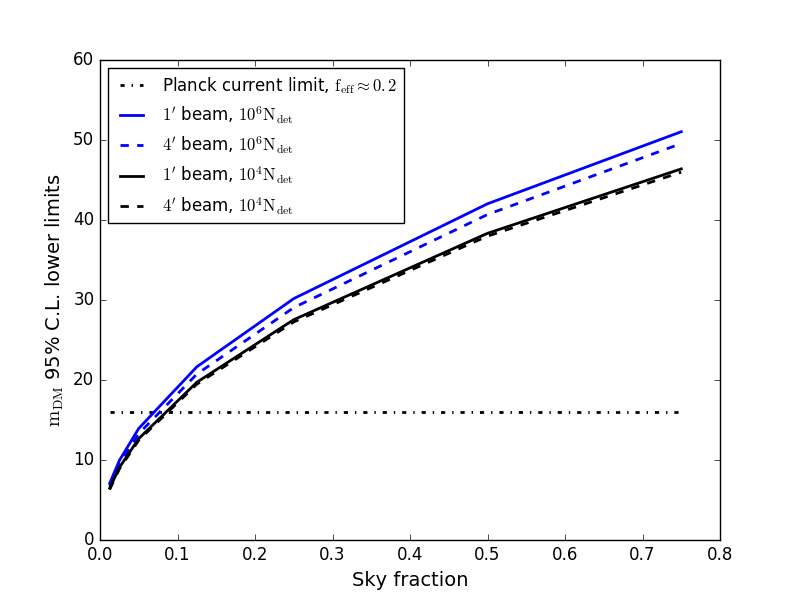
\includegraphics[width=0.7\textwidth]{DarkEnergy/DM_annihilation_CMBS4.png}
\caption{95 \% CL upper limit on $m_{\rm DM}$ in GeV as a function of sky coverage, $f_{\rm sky}$.
The blue/black lines correspond to $10^6$/$10^4$ detectors. The solid/dashed lines correspond to 1'/4' beams.
The dashed/dotted lines show the limit from Planck for a thermal cross section and $100\%$ of the energy absorbed by the plasma (it was expected from Fisher forecasts and then confirmed by the Planck collaboration measurements).}\label{fig:DM_annihilation}
\end{center}
\end{figure}

Dark-matter annihilation also leads to growing ionization fraction perturbations and amplified small-scale cosmological perturbations, leaving an imprint on the CMB bispectrum \cite{Dvorkin:2013cga}.

%
\section{Other types of Dark Matter Interactions}
%
Near the epoch of CMB last scattering, dark matter accounts for about $65\%$ of the energy budget of the Universe, hence making the CMB a particularly good probe of potential new physics in the dark matter sector. Of particular relevance to CMB-S4 studies, the presence of new dark matter interactions with light degrees of freedom \cite{Goldberg:1986nk,Carlson:1992fn,Gradwohl:1992ue,Machacek:1994vg,deLaix:1995vi,AtrioBarandela:1996ur,Boehm:2001hm,Foot:2004pa,Green:2005fa,Profumo:2006bv,Mangano:2006mp,Ackerman:2008gi,ArkaniHamed:2008qn,Feng:2009mn,Serra:2009uu,Bringmann:2009vf,Kaplan:2009de,McDermott:2010pa,Kaplan:2011yj,Aarssen:2012fx,Diamanti:2012tg,Baldi:2012ua,Cline:2012is,CyrRacine:2012fz,Fan:2013yva,Fan:2013tia,Cyr-Racine:2013fsa,Bringmann:2013vra,Wilkinson:2013kia,Dvorkin:2013cea,Boehm:2014vja,Wilkinson:2014ksa,Escudero:2015yka,Chu:2014lja,Archidiacono:2014nda,Buen-Abad:2015ova,Lesgourgues:2015wza} can leave subtle imprints on the temperature and polarization CMB power spectra. The introduction of such non-minimal dark matter models has been primarily (but not exclusively) motivated in the literature by potential shortcomings of the standard cold dark matter scenario at small sub-galactic scales \cite{deBlok:1997zlw,Klypin:1999uc,Moore:1999nt,Zavala:2009ms,Oh:2010ea,BoylanKolchin:2011de,Papastergis:2011xe,Walker:2011zu,Pawlowski:2013kpa,Klypin:2014ira,Oman:2015xda,Papastergis:2014aba}. While these issues are far from settled, they motivate the search for other non-minimal dark matter signatures in complementary data sets (such as the CMB) that could indicate whether or not dark matter can be part of the solution. 

\subsection{Dark Matter-Baryon Scattering}

A possible dark matter scenario is that in which dark matter scatters off baryons in the early universe. 
In this scenario, there is a drag force produced by the baryons on the dark matter fluid, which affects the CMB temperature and polarization power spectra and the matter power spectrum.
Ref. \cite{Dvorkin:2013cea} has done a model-independent analysis on the Dark Matter-Baryon interactions using CMB temperature data from the {\it Planck satellite}, and the Lyman-$\alpha$ forest data from the {\it Sloan Digital Sky Survey}, as a tracer of the matter fluctuations. This analysis suggests that the constraints could become significantly better with better temperature data on small scales, and additional polarization data at large and small scales. Therefore, an experiment such as CMB-S4 would have a large impact on these constraints.

\subsection{Dark Matter-Dark Radiation Interaction}
Dark matter interacting with light (or massless) dark radiation  has been put forward \cite{Buen-Abad:2015ova,Lesgourgues:2015wza} as a potential solution to the small discrepancy between the amplitude of matter fluctuations inferred from CMB measurements and those inferred from cluster number counts and weak lensing measurements. CMB-S4 measurements of the lensing power spectrum have the potential to significantly improve constraints on dark matter interacting with light degrees of freedom in the early Universe.

The key equations governing the evolution of cosmological fluctuations for this broad class of non-minimal dark matter models are presented in Ref.~\cite{Cyr-Racine:2015ihg}. Essentially, the new dark matter physics enters entirely through the introduction of dark matter and dark radiation opacities, which, similarly to the photon-baryon case, prohibit dark radiation free-streaming at early times and provides a pressure term that opposes the gravitational growth of dark matter density fluctuations. The impact of this new physics on CMB fluctuations has been studied in detail in Ref.~\cite{Cyr-Racine:2013fsa} and we briefly review it here. First, the presence of extra dark radiation mimics the presence of extra neutrino species and affects the expansion history of the Universe, possibly modifying the epoch of matter-radiation equality, the CMB Silk damping tail, and the early Integrated Sachs-Wolfe effect. However, unlike standard free-streaming neutrinos, the dark radiation forms a tightly-coupled fluid at early times, leading to distinct signatures on CMB fluctuations which include a phase and amplitude shift of the acoustic peaks (see e.g. Ref.~\cite{Bashinsky:2003tk,Cyr-Racine:2013jua,Follin:2015hya}). Second, the dark radiation pressure prohibits the growth of interacting dark matter fluctuations on length scales entering the causal horizon before the epoch of dark matter kinematic decoupling. This weakens the depth of gravitational potential fluctuations on these scales, hence affecting the source term of CMB temperature fluctuations. Finally, the modified matter clustering in the Universe due to nonstandard dark matter properties will affect the lensing of the CMB as it travel from the last-scattering surface to us. For interacting dark matter models that are still allowed by the current Planck data, this latter effect is where CMB-S4 can significantly improve the constraints on these non-minimal theories.

Given the large array of possible dark matter theories to constrain, we use the Effective THeory Of Structure formation (ETHOS) \cite{Cyr-Racine:2015ihg} to systematically parametrize the deviations from standard cold dark matter. Within ETHOS, the impact of having all or a fraction of dark matter interacting with dark radiation can be captured with a handful of ``effective'' parameters which entirely determine the structure of the linear matter power spectrum. The most relevant parameters are \cite{Cyr-Racine:2015ihg}
%
\begin{equation}
\Xi_{\rm ETHOS} = \Big\{\omega_{\rm DR},f_{\rm int}, \{a_n,\alpha_l\} \Big\},
\end{equation}
%
where $\omega_{\rm DR} = \Omega_{\rm DR}h^2$ is the physical energy density in dark radiation in units of the critical density of the Universe, $f_{\rm int}$ is the fraction of the total dark matter density that interacts with dark radiation, and where $a_n$ and $\alpha_l$ are parameters describing the size of the interaction cross section and its angular dependence, respectively. The coefficients $a_n$ enter directly into the calculation of the dark matter drag opacity $\dot{\kappa}_\chi$ as:
%
\begin{equation}
\dot{\kappa}_\chi =- \omega_{\rm DR} \sum_n \left(\frac{2+n}{3}\right)a_n \frac{(1+z)^{n+1}}{z_{\rm D}^n},
\end{equation}
%
where $z_{\rm D}$ is a normalization scale. Choosing the latter to correspond to the dark matter decoupling redshift ensures that the $a_n$ coefficients are of order unity. The index $n$ is directly related to the nature of the physical process coupling dark matter and dark radiation: a non-vanishing $a_n$ coefficient implies a scattering process characterized by the matrix element $|\mathcal{M}|^2 \propto (p_{\rm DR}/m_\chi)^{n-2}$, where $p_{\rm DR}$ is the incoming momentum of the dark radiation and $m_\chi$ is the dark matter mass. Since the decoupling of dark matter from dark radiation is given by the approximate criterion $-\dot{\kappa}_\chi = H$, the magnitude of the ETHOS coefficients $a_n$ set the scale at which the CMB lensing power spectrum departs from its $\Lambda$CDM counterpart.  We use the ETHOS parametrization to illustrate that CMB-S4 can provide competitive constraints on partially interacting dark matter theories.

We illustrate in Fig.~\ref{fig:Cls_phi_PIDM} the impact of different interacting dark matter models on the CMB lensing power spectrum. In the top panel, we show four partially-interacting dark matter models parametrized by their ETHOS opacity coefficient and for which only $5\%$ of the total amount of dark matter is interacting. We display the fractional difference between the ETHOS models and a standard $\Lambda$CDM model with vanishing neutrino mass. For comparison, we also illustrate the difference for a standard massive neutrino $\Lambda$CDM model with $\sum m_\nu = 0.06$ meV.  Interestingly, the damping of the lensing power spectrum has a different shape than that caused by massive neutrinos. Given the expected performance of CMB-S4 in measuring the lensing power spectrum, all the model illustrated there (which are currently allowed by Planck data) could be ruled out, significantly improving our knowledge about interacting dark matter. The lower panel of Fig.~\ref{fig:Cls_phi_PIDM} is similar, but illustrates how the fractional difference in the CMB lensing power spectrum is affected as the fraction of interacting dark matter is varied from $5$ to $2$ percents. Again, this illustrates that CMB-S4 can provide very tight constraints on the fraction of interacting dark matter.

%
\begin{figure}[htbp!]
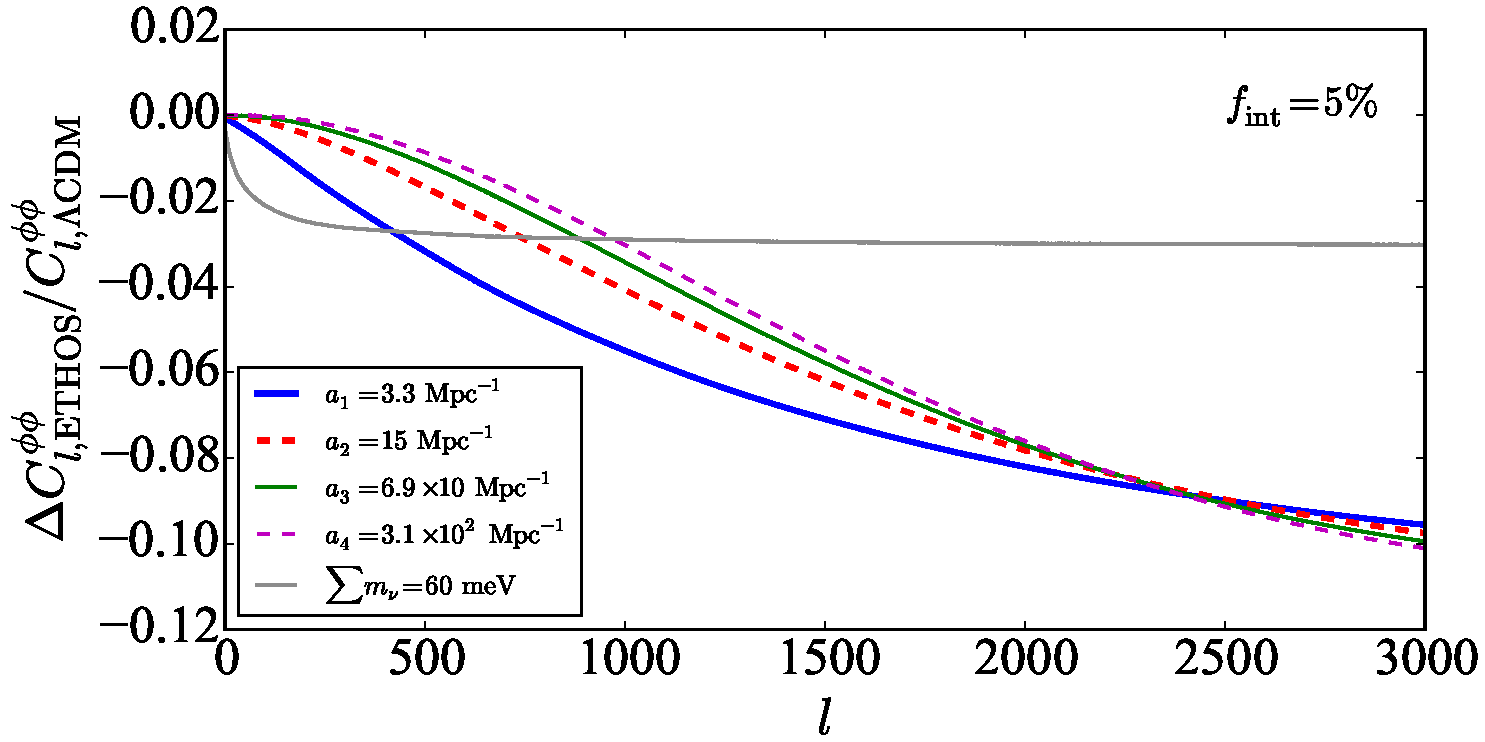
\includegraphics[width=\textwidth]{DarkEnergy/ClsPP_ETHOS_a_n.pdf}\\
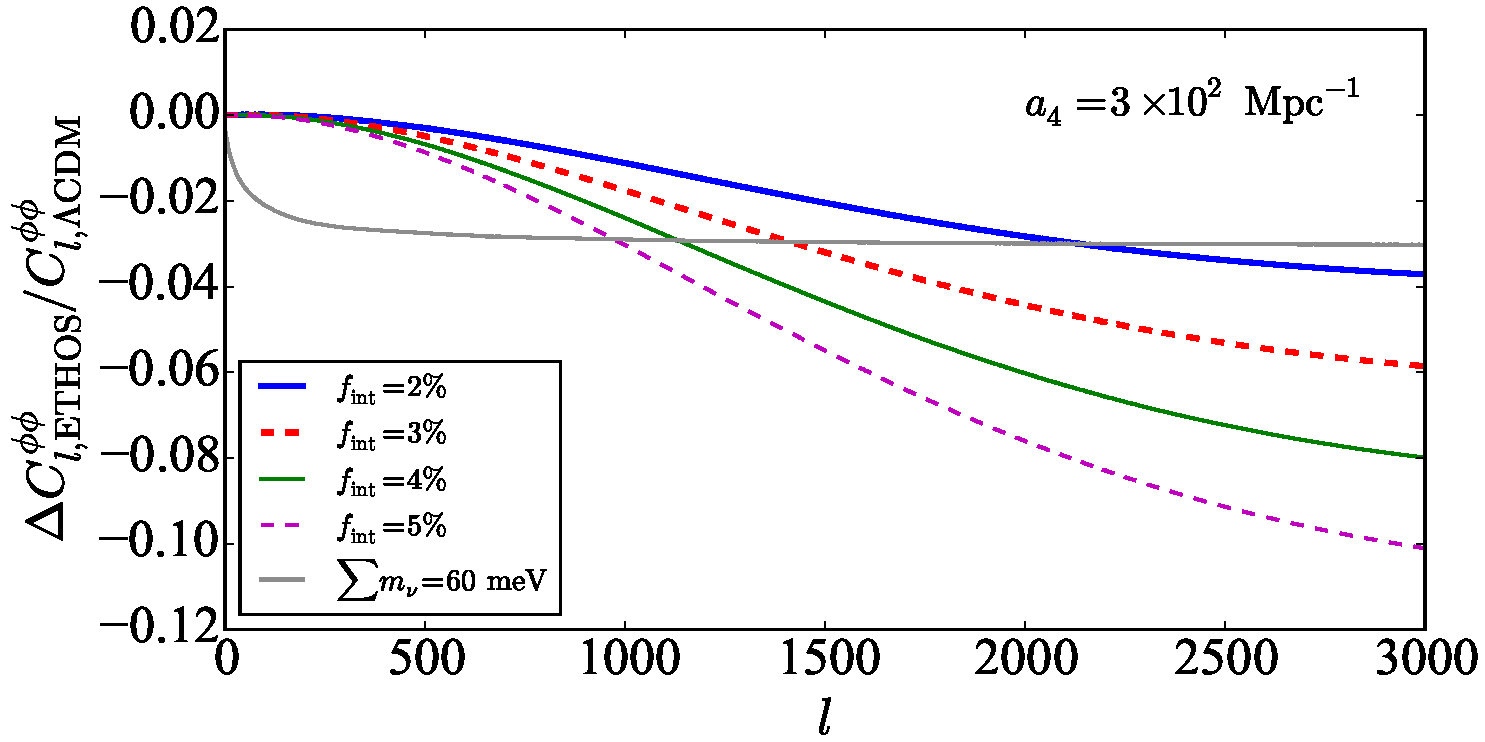
\includegraphics[width=\textwidth]{DarkEnergy/ClsPP_ETHOS_f_int.pdf}
\caption{\emph{Top panel}: Fractional difference of the CMB lensing spectrum between a standard $\Lambda$CDM model (with massless neutrinos) and four different ETHOS models with opacity coefficients $a_n$ given in the legend. In all models shown, $5\%$ of the dark matter is allowed to interact with dark radiation. For comparison, we also display a standard massive neutrino model with $\sum m_\nu =0.06$ meV. \emph{Lower panel}: Similar to the top panel, but we now vary the fraction of dark matter that can interact with dark radiation, for a fixed opacity coefficient of $a_4 = 3\times 10^2$ Mpc$^{-1}$. }\label{fig:Cls_phi_PIDM}
\end{figure}
%

Since non-standard dark matter models affect primarily the large CMB lensing multipoles, the constraining power of CMB-S4 on interacting dark matter is largely independent of the specific choice of $\ell_{\rm min}$. We foresee that the main difficulty in constraining non-standard dark matter theories with CMB-S4 will be the proper modeling of non-linearities in the matter power spectrum, which are quite important for $\ell > 500$. We note that recent progress has been made in this direction \cite{Vogelsberger:2015gpr}.


\section{Axion Dark Matter}

\subsection{Constraints on cold axion energy density}
The QCD axion and other axion-like particles (ALPs), if stable on cosmological timescales, can contribute to the DM density. Along with thermal WIMPs, they are a well-motivated DM candidate (see Ref.~\cite{Marsh:2015xka} for a recent review).

Non-thermally produced ultralight axions (ULAs) with masses in the range $10^{-33}~{\rm eV}\leq m_{a}\leq 10^{-20}~{\rm eV}$ are well motivated by string theory, can contribute to either the dark matter or dark energy components of the Universe, depending on their masses, and are distinguishable from DE and CDM in cosmological observables. The current best constraints from the primary CMB TT power, and WiggleZ galaxy redshift survey were made in \cite{Hlozek:2014lca}. Our fiducial axion energy density is chosen to be consistent with these constraints. 

The degeneracies of the axions with other cosmological parameters, such as $N_\mathrm{eff}$ or $m_\nu$, vary depending on the axion mass (see Fig.~\ref{fig:axions}, right panel). Dark energy-like axions with masses around $10^{-33}~{\rm eV}$ change the late-time expansion rate and therefore the sound horizon, changing the location of the acoustic peaks. This has degeneracies with the matter and curvature content. 
Heavier axions ($m_a \gtrsim 10^{-26}~{\rm eV}$) affect the expansion rate in the radiation era and reduce the angular scale of the diffusion distance, leading to a boost in the higher acoustic peaks, which has a degeneracy with $N_{\rm eff}$. 

In both of these cases, improved errors on the temperature and polarization power spectrum, coupled with constraints on the Hubble constant (for the lightest axions) from Baryon Acoustic Oscillations, lead to improvements in the error on allowed axion energy density of a factor of three from these spectra alone. 

In the matter power spectrum, and thus CMB lensing power, light axions suppress clustering power, suggesting a degeneracy with effects of massive neutrinos that must be broken to make an unambiguous measurement of neutrino mass using the CMB. The above-mentioned effects in the expansion rate break this degeneracy for some axion masses. There remains a significant degeneracy between axions and massive neutrinos $m_a=3\times 10^{-29}\text{ eV}$ and $\Sigma m_\nu=60\text{ meV}$. Effort should be made to break this degeneracy and distinguish the effects of non-thermal axions from massive neutrinos for an unambiguous detection of neutrino mass using the CMB. 

\begin{figure}[t] 
\begin{center} 
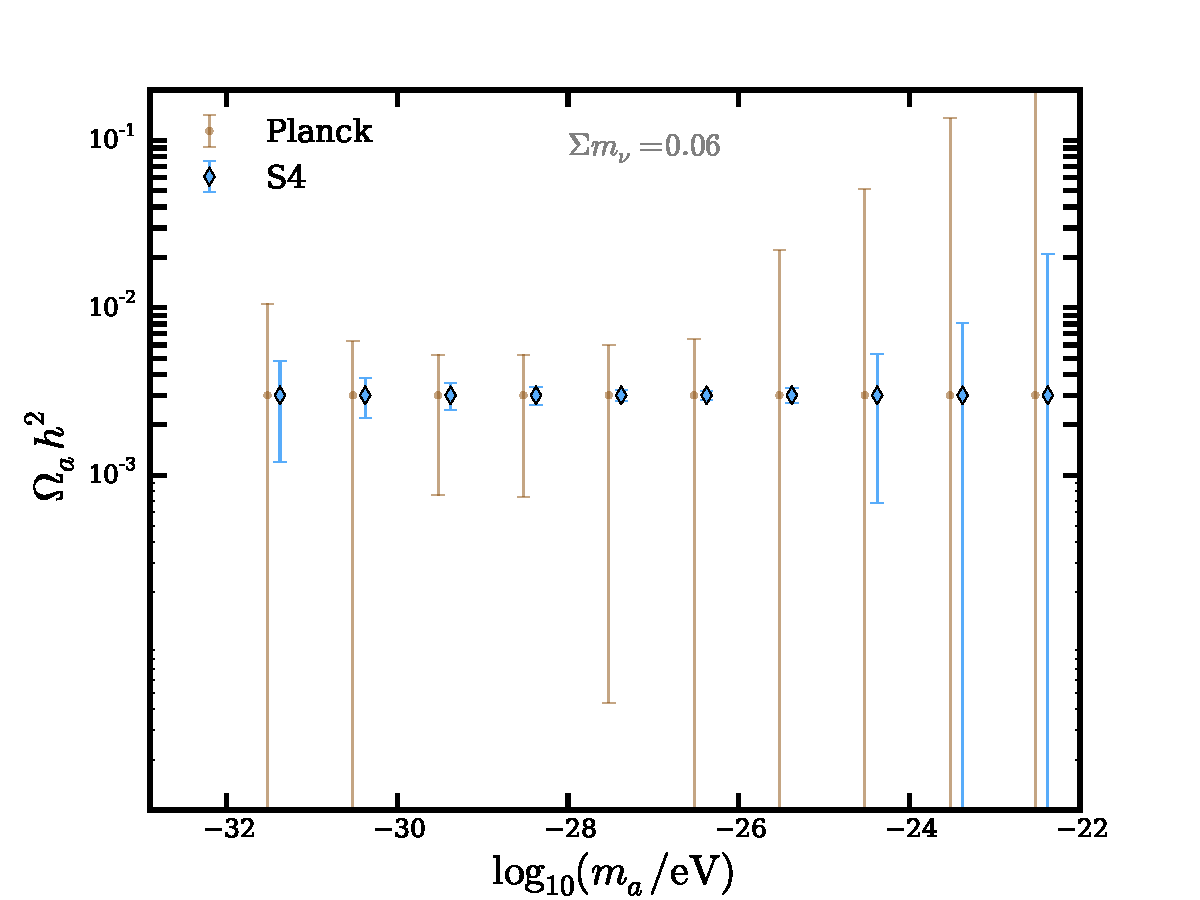
\includegraphics[width=0.49\textwidth]{DarkEnergy/Log_constraints_axions_s4.pdf}
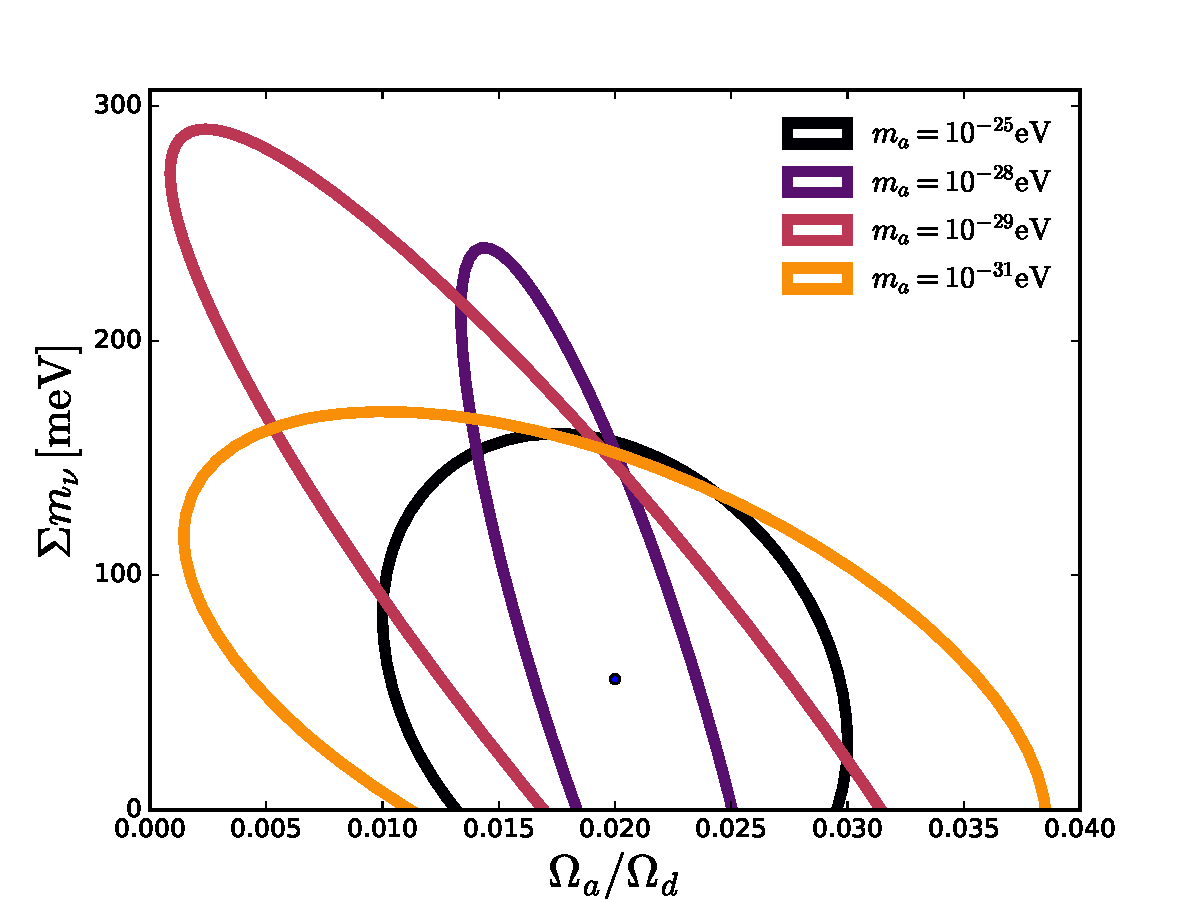
\includegraphics[width=0.49\textwidth]{DarkEnergy/s4_frac_omnuh2.pdf}
\caption{\textbf{Left:} Constraints on the axion energy density as a function of axion mass at fixed neutrino mass $\Sigma m_\nu = 0.06~\rm{eV}$ (errorbars) and marginalising over the neutrino mass (shaded error bars), for Planck Blue Book constraints (brown) and a CMB-S4-like survey (blue). Over the `fuzzy' dark matter region ($-28 < \log(m_a/\mathrm{eV}) < -25$, CMB-S4 allow for percent-level constraints on an axion component, improving significantly on current constraints. For the same range of masses, the degeneracy is weakest with massive neutrinos - the bands shown when marginalising over the neutrino error are not much larger than the case where the neutrino mass is fixed. \textbf{Right:} Degeneracy of axions with massive neutrinos. There is a significant degeneracy for $m_a=3\times 10^{-29}\text{ eV}$ and $\Sigma m_\nu=60\text{ meV}$. Figure from Hlo\v{z}ek et al. (prep).
\label{fig:axions}}
\end{center}       
\end{figure}       

We show the forecasted constraints on the axion energy density from CMB-S4 including lensing in the left panel of Figure~\ref{fig:axions} (for fixed neutrino mass of $\Sigma m_\nu = 0.06~\rm{eV}$). Adding in information from the lensing reconstruction using CMB-S4 will improve constraints on axion DM significantly. A percent-level measurement of the lensing deflection power at multipoles $\ell > 1000$ leads to an improvement in the error on the axion energy density of a factor of eight relative to the current Planck constraints, for an axion mass of $m_a=10^{-26}~{\rm eV}$.    This represents an ability to test the component nature of dark matter, and thus the CDM paradigm, at the percent level. Furthermore, since $\Omega_a\propto f_a^2$ this improves the expected constraint on the axion decay constant from $10^{17}\text{ GeV}$ with Planck to $10^{16}\text{ GeV}$ with CMB-S4, testing the predictions of the ``string axiverse’’ scenario~\cite{Arvanitaki:2009fg}. 

Planck is degenerate with CDM at $m_a=10^{-24}\,\mathrm{eV}$, and only has weak constraints at $m_a=10^{-25}\,\mathrm{eV}$. CMB-S4 introduces a $5\sigma$ constraint at $m_a=10^{-25}\,\mathrm{eV}$, and improves the lower bound on DM particle mass to $m_a=10^{-23}\,\mathrm{eV}$ and fractions O(10\%). However, realising this requires improved understanding of non-linear clustering in axions \cite{Marsh:2016vgj}.

\subsection{Axion Isocurvature \label{axion_iso}}

A key axion parameter is the symmetry breaking scale, $f_a$. If $H_I/2\pi<f_a$, the axion DM acquires \emph{uncorrelated isocurvature perturbations} (e.g. Refs.~\cite{Axenides:1983hj,Fox:2004kb,Hertzberg:2008wr}).\footnote{We ignore the case where $H_I/2\pi>f_a$, since no isocurvature initial conditions are excited. The limit $r_{0.05}<0.12$ implies that isocurvature is produced if $f_a>1.8\times 10^{13}\text{ GeV}$. This accounts for the QCD axion in the ``anthropic'' window (roughly half of the allowed range of $f_a$ on a logarithmic scale), axions with GUT scale decay constants (such as string axions~\cite{Svrcek:2006yi,Arvanitaki:2009fg}) and axions with lower $f_a$ in models of low-scale inflation.} The uncorrelated CDM isocurvature amplitude is bounded by \emph{Planck} to be $A_I/A_s<0.038$ at 95\% C.L.~\cite{Ade:2015lrj}. We performed a forecast for CMB-S4: the isocurvature limit will be improved by a factor of approximately five compared to \emph{Planck}, allowing for detection of axion-type isocurvature at 2$\sigma$ significance in the region $0.008<A_I/A_s<0.038$.

The axion isocurvature amplitude is:
\begin{equation}
A_I = \left(\frac{\Omega_a}{\Omega_d}\right)^2\frac{(H_I/M_{\rm pl})^2}{\pi^2(\phi_i/M_{\rm pl})^2} \, .
\label{eqn:iso_amplitude}
\end{equation}
The initial axion displacement, $\phi_i$, fixes the axion relic abundance such that $\Omega_a=\Omega_a (\phi_i,m_a)$~\cite{Preskill:1982cy,Abbott:1982af,Dine:1982ah,Turner:1983he,Steinhardt:1983ia,Marsh:2010wq}. Thus, if the relic density and mass can be measured by independent means, \emph{a measurement of the axion isocurvature amplitude can be used to measure the energy scale of inflation, $H_I$}

If the QCD axion is all of the DM, axion direct detection experiments can be used in conjunction with CMB-S4 to probe $H_I$ in the range
\begin{equation}
 2.5\times 10^6\lesssim H_I/\text{GeV}\lesssim 4\times 10^9\, 
\text{(QCD axion + direct detection)}\, \,
\end{equation}
This is demonstrated in Fig.~\ref{fig:qcd_isocurvature} (left panel) for the case of ADMX~\cite{Asztalos:2009yp} (in operation), and CASPEr~\cite{Budker:2013hfa} (proposed), where we have used the standard formulae relating the QCD axion mass and relic abundance to the decay constant (e.g. Ref.~\cite{Fox:2004kb}).\footnote{In simple models of inflation, the high-$f_a$ QCD axion is incompatible with detection of tensor modes~\cite{Fox:2004kb,Hertzberg:2008wr,Visinelli:2014twa,Marsh:2014qoa,Visinelli:2014twa}, although non-standard cosmic thermal histories of PQ breaking mechanisms can lift constraints , e.g. \cite{Higaki:2014ooa,Fairbairn:2014zta,Nomura:2015xil}.} \emph{Combining axion DM direct detection with CMB-S4 isocurvature measurements allows a unique probe of low-scale inflation, inaccessible to searches for tensor modes.}

\begin{figure*}[htbp!]
\begin{center}
$\begin{array}{@{\hspace{-0.4in}}c@{\hspace{0.1in}}c@{\hspace{0.1in}}c@{\hspace{+0.1in}}}
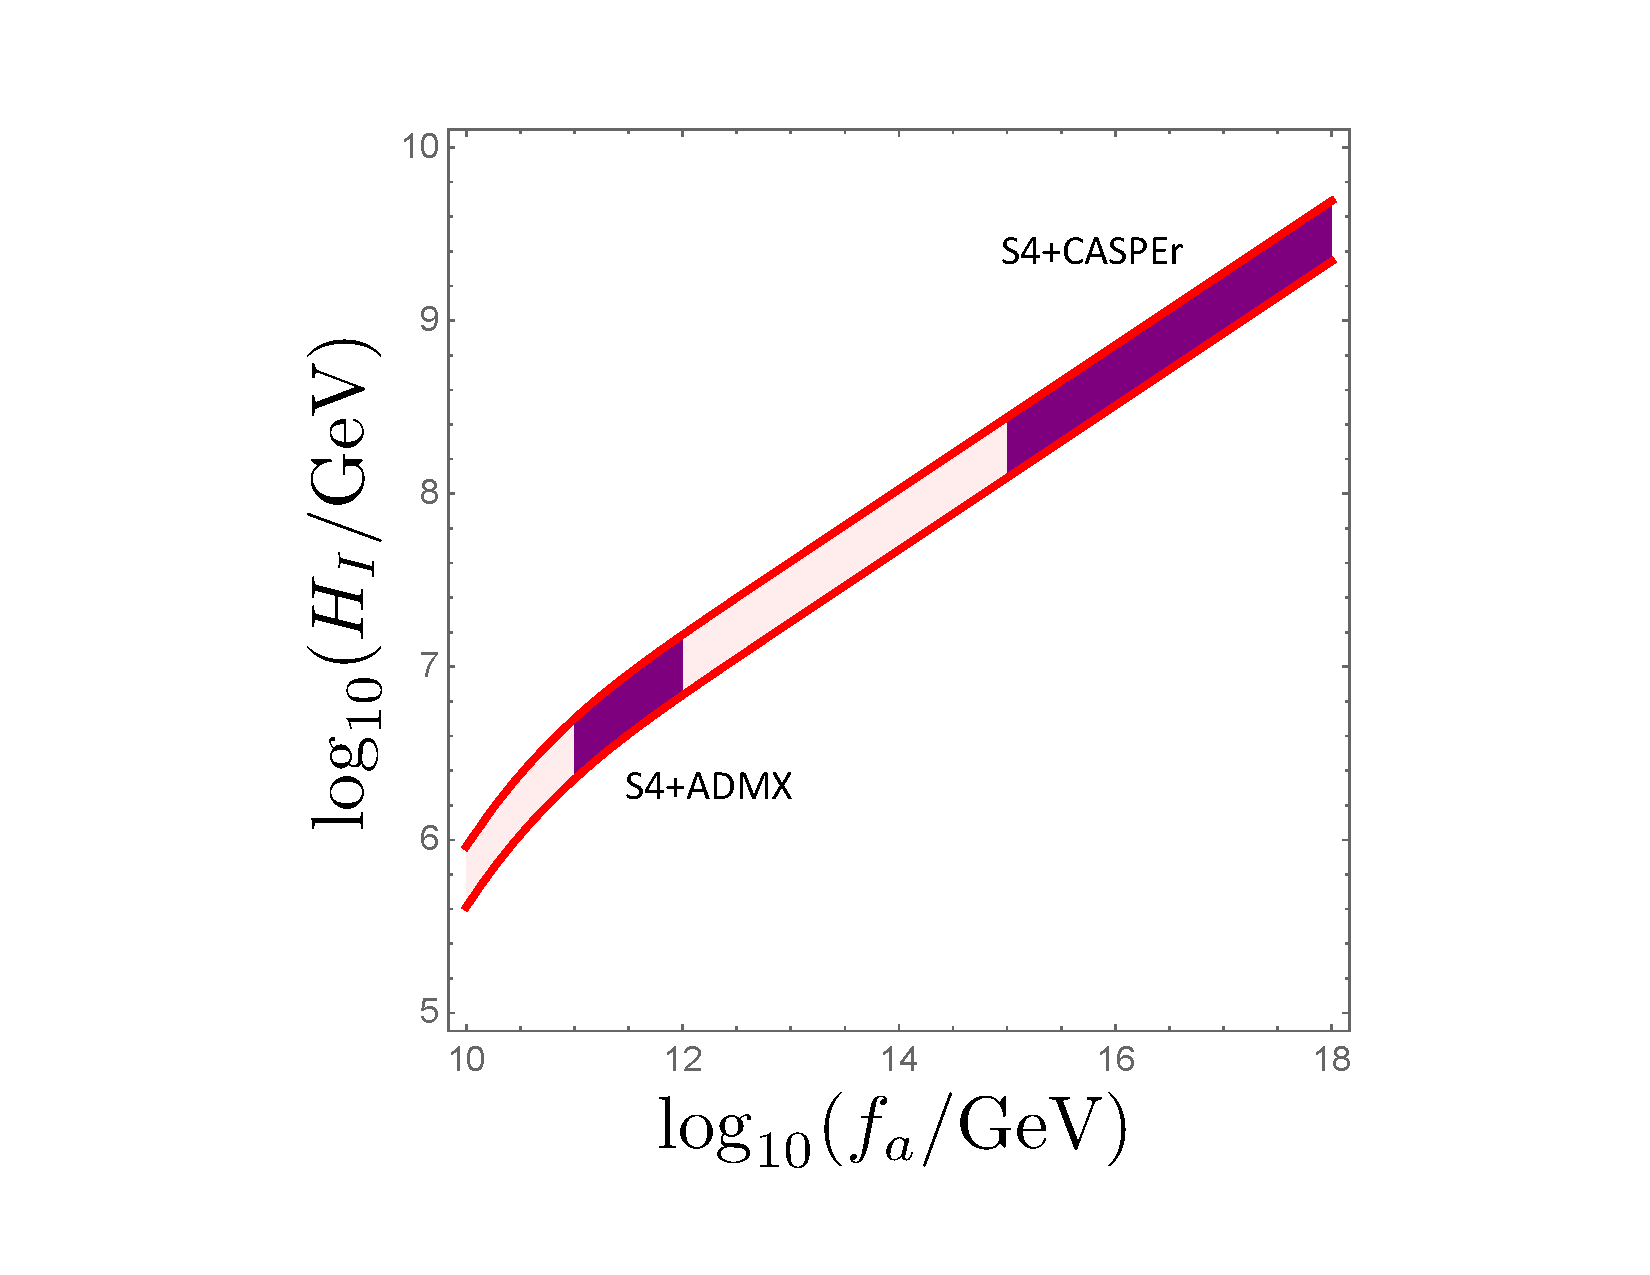
\includegraphics[width=0.3\textwidth]{Inflation/admx_casper_labelled.pdf} &
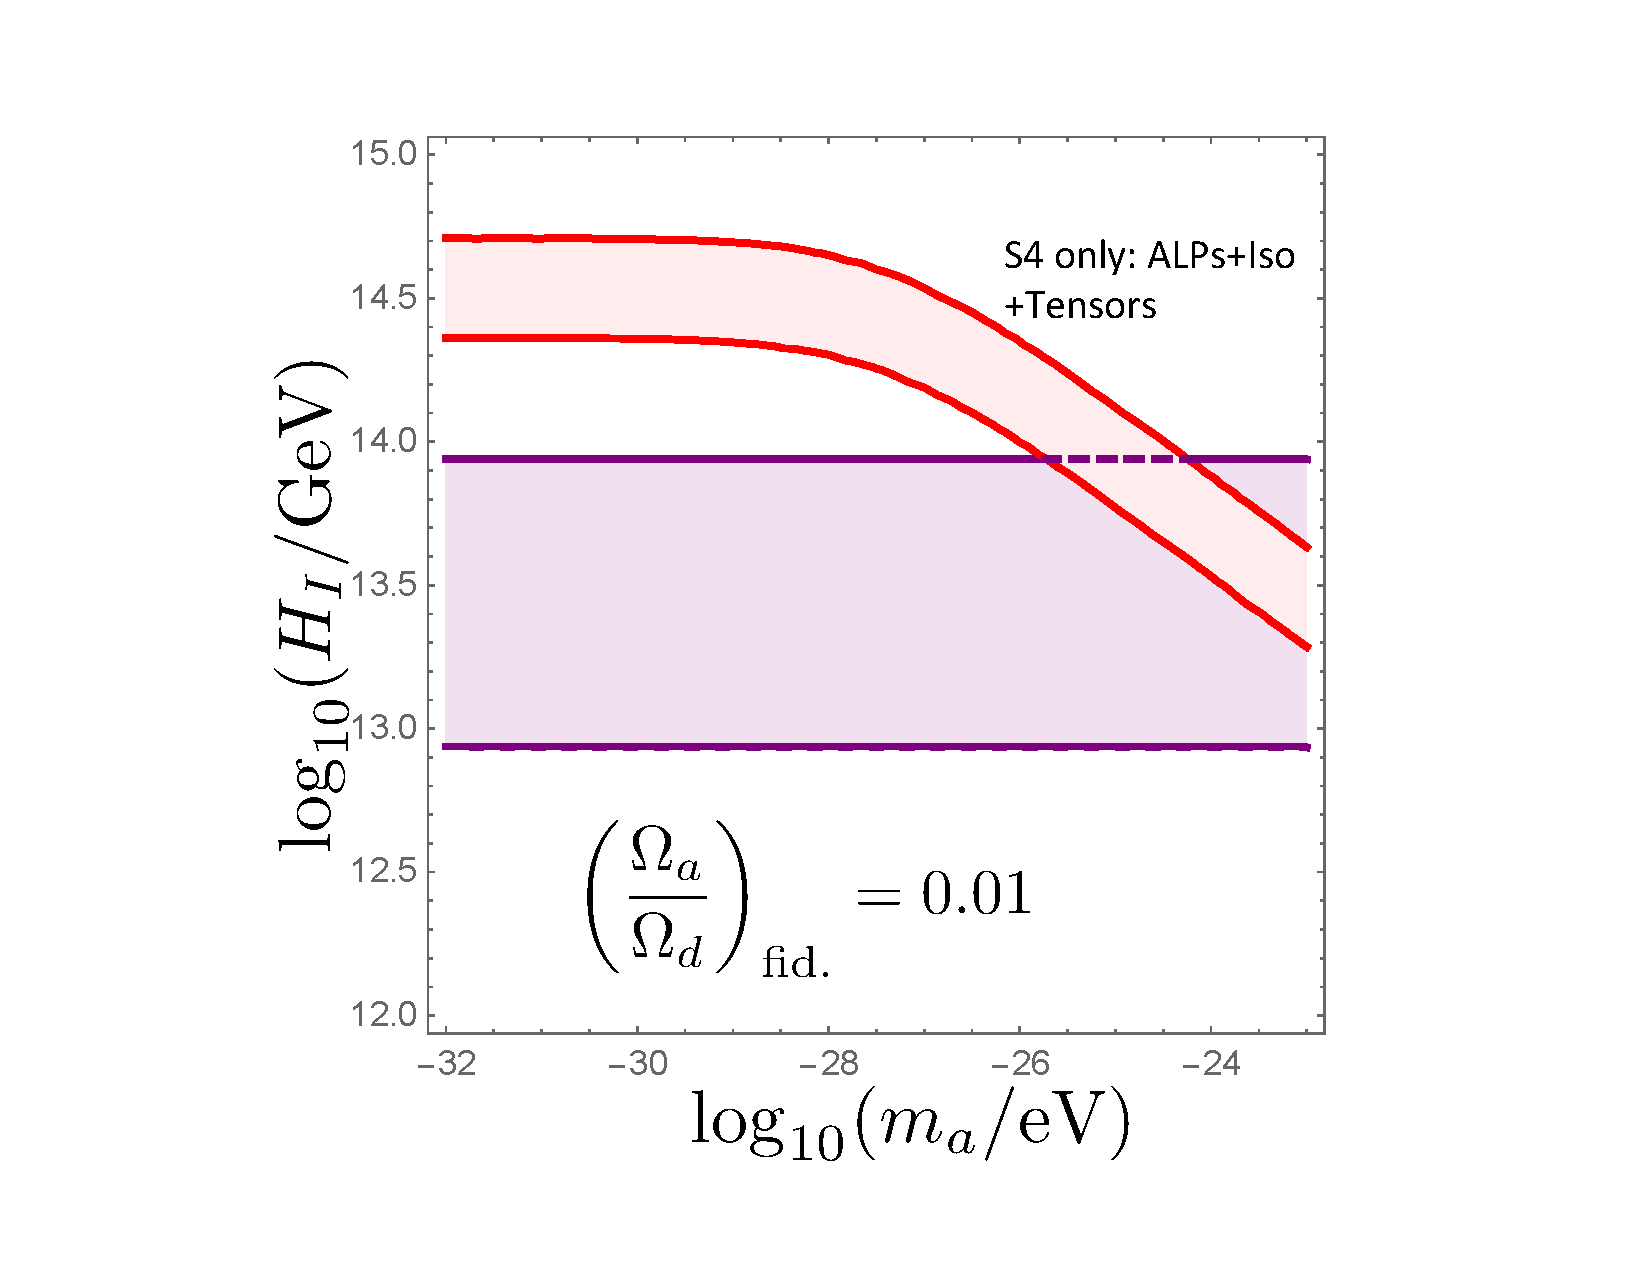
\includegraphics[width=0.3 \textwidth]{Inflation/alp_iso_labelled.pdf} &
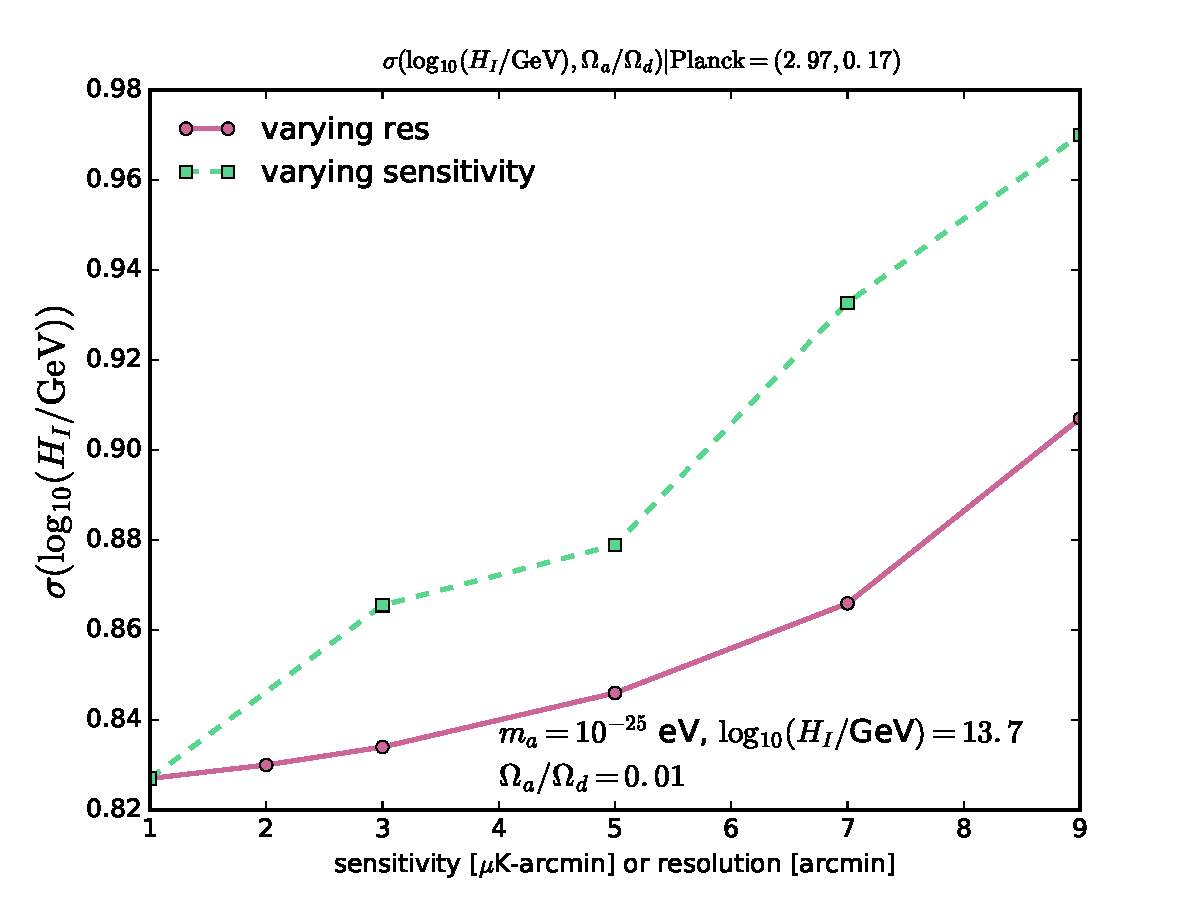
\includegraphics[width=0.4\textwidth]{Inflation/ALP_iso_mass_m25_Hi_sensitivity_resolution.pdf}
 \end{array}$
 \end{center}
 \caption{Axion dark matter isocurvature. Red bands in the left and middle panels show the isocurvature amplitude consistent with Planck and detectable with CMB-S4. \textbf{Left Panel:} The QCD axion: measuring the energy scale of inflation with CMB-S4+axion direct detection. Here we restrict axions to be all of the DM. The purple regions show the range of $f_a$ accessible to axion direct detection experiments. Combining ADMX~\cite{Asztalos:2009yp} (in operation), CASPEr~\cite{Budker:2013hfa} (proposed), and CMB-S4 it is possible to measure $4\times 10^5\lesssim H_I/\text{GeV}\lesssim 4\times 10^9$. \textbf{Middle Panel:} ALPs - a combination measurement using CMB-S4 alone. Assuming 1\% of the total DM resides in an ultralight axion, the mass and axion density can be determined to high significance using, for example, the lensing power. The isocurvature amplitude can also be determined, allowing for an independent determination of $H_I$ in the same regime as is accessible from tensor modes (purple band). \textbf{Right Panel:} We vary $H_I$ directly around a fiducial model of $H_I/\text{GeV} = 10^{13.7}$ for axions of mass $10^{-25} \mathrm{eV}$ making up 1\% of the total dark content, for a range of possible CMB-S4 survey parameters. While the error degrades as the resolution and sensitivity are worsened, this degradation is small compared to the factor of three improvemement in the error moving from Planck to CMB-S4.}
\label{fig:qcd_isocurvature}
\end{figure*} 
We now consider isocurvature in ultralight ALPs (ULAs, see e.g. Refs.~\cite{Marsh:2013taa,Marsh:2014qoa}). ULA DM has a number of distinctive features in large scale structure and the CMB~\cite{Hlozek:2014lca,Marsh:2013ywa}. For ULAs with $10^{-32}\lesssim m_a/\text{eV}\lesssim 10^{-23}$ a DM fraction of $\Omega_a/\Omega_d$ in the range of 1\% is consistent with \emph{Planck}~\cite{Hlozek:2014lca} and high-$z$ galaxy formation~\cite{Bozek:2014uqa,Schive:2015kza}, yet can be distinguished from pure CDM using CMB-S4 lensing power at $>2\sigma$ (depending on the ULA mass, Sec.~\ref{sec:uladiabat}). Fig.~\ref{fig:qcd_isocurvature} (middle panel) shows isocurvature constraints possible with CMB-S4, compared to tensor constraints. We fix the fiducial ULA fraction to 1\%, such that $\Omega_a$ and $m_a$ can be separately measured using the CMB-S4 lensing power, and thus using Eq.~(\ref{eqn:iso_amplitude}) a measurement of $A_I$ is a measurement of $H_I$. 

In contrast to the QCD axion, there are masses, $m_a\lesssim 10^{-26}\text{ eV}$, for which tensor modes impose a stronger constraint on $H_I$ than isocurvature (such that isocurvature in these ALPs would be undetectably small). However, there are also regions of overlap between possible tensor and isocurvature measurements. Using CMB-S4 in these regions, it is possible to make a combination measurement of isocurvature and axion parameters, giving an independent measurement of $H_I$:
\begin{equation} 2.5\times 10^{13}\lesssim H_I/\text{GeV}\lesssim 10^{14}\,
\text{(ultralight ALPs, CMB-S4 alone)}\,\,.
\end{equation}
This applies to ALPs in the mass range $10^{-26}\lesssim m_a/\text{eV}\lesssim 10^{-23}$, where effects on lensing of a 1\% axion fraction can be distinguished from CDM. \emph{Detecting isocurvature and lensing effects from ULAs using CMB-S4 can provide a measurement of $H_I$ complementary to searches for tensor modes.}%\footnote{We note that obtaining a 1\% fraction in such ALPs requires $f_a\gg 1.8\times 10^{13}\text{ GeV}$, and so isocurvature in ULA DM is guaranteed.}

\section{Summary}
Determining the nature of dark matter remains one of the main goals of the current cosmological epoch. CMB-S4 will provide not only a handle on distinguishing between different models of DM annihilation and other models of DM interaction, but will also place extremely tight constraints on axions and axion-like particles. This will allow CMB-S4 to probe the dark sector and reduce the boundary of ignorance on (or detect!) this important cosmological component.

